In this chapter, we present the technical background needed to understand the proposed distributed computing architecture and position it within the existing literature.

\section{The ASA Project}

\gls{asa} is a software ecosystem created for the modeling and simulation of military operational scenarios to support the development of tactics and procedures in the aerospace context for the Brazilian Air Force \parencite{dantas2025asa}. It supports scenario modeling and both simulation execution and output analysis via a custom python library named Asapy \parencite{dantas2024asapy}, providing the Brazilian Air Force's higher command with quantitative and statistically robust analyses of outcomes of aerospace defense scenarios. The architectural solution addressed in this thesis concerns a specific bottleneck: while \gls{asa} excels at scenario execution, post-processing of large result volumes becomes inefficient when handled serially on a single machine. If the analyst must manually retrieve, structure, and aggregate raw results after each batch, the overall workflow becomes slower and less scalable.

The core contribution of this work is to improve simulation outputs are transformed into analytical products through distributed post-processing, without requiring changes to the core simulation logic. 

\section{Capacity-Based Planning (CBP)}

\gls{cbp} is a defense-planning approach centered on the capabilities required to accomplish missions under multiple plausible scenarios, rather than on a single predefined threat. In this perspective, the planning process asks which operational effects must be achieved and which combinations of systems, doctrine, personnel, and infrastructure are needed to achieve them robustly across different future situations. As discussed by \textcite{davis2002cbp}, \gls{cbp} is particularly useful when uncertainty is high and when strategic decisions must remain valid under changing technological, political, and operational conditions.


From an analytical standpoint, \gls{cbp} depends on methods capable of comparing alternatives under uncertainty. That is why it is commonly associated with techniques such as Delphi-based elicitation \parencite{egfjord2020delphi}, and modeling and simulation. In military environments, those techniques are not merely auxiliary tools; they are part of the evidence-generation process through which planners justify capability-development decisions \parencite{hodicky2020cbp}.

In an air-defense context, \gls{cbp} helps transform broad strategic concerns into concrete analytical questions. Instead of asking only which isolated system should be acquired or upgraded, planners may ask which capability mix is required to improve survivability, interception success, warning time, operational flexibility, or resource efficiency. This makes the planning process inherently scenario-based: the same force structure may perform differently depending on radar placement, enemy behavior, rules of engagement, and coordination between assets.

Air-defense planning therefore benefits from analytical environments in which multiple scenarios can be generated, executed, and compared in a structured manner. This is especially important when force design decisions must balance offensive and defensive investments, doctrinal alternatives, and constrained resources. In such cases, \gls{cbp} works as a bridge between high-level strategic questions and operationally grounded evaluations \parencite{davis2002cbp,hodicky2020cbp}.

\section{Modeling and Simulation (M\&S)}

\gls{ms} refers to the combined use of mathematical and computational representations to abstract real-world systems and replicate their behavior under controlled conditions. A model encodes the essential elements, relationships, and rules that govern a system's dynamics, while a simulation executes that model to generate outcomes over time. \gls{ms} has become a fundamental tool across engineering, operations research, and defense, enabling the study of complex systems that are too costly, dangerous, or time-consuming to experiment with directly. By abstracting reality into a computable form, \gls{ms} allows analysts to pose hypothetical questions, observe consequences, and reason about system behavior before implementing decisions in the real world.

In the context of operational planning and defense analysis, \gls{ms} serves as a bridge between strategic concepts and measurable operational effects. Rather than relying solely on intuition or historical precedent, planners can construct detailed scenarios, execute them repeatedly under different parameter values, and extract empirical evidence about how systems respond to changing conditions. This evidence generation process is essential for decisions that involve high costs, significant uncertainties, and interdependencies among many variables, precisely the characteristics of capability-based planning in complex domains such as aerospace defense.

Defense-oriented simulation has long been used for analysis, research and development, test and evaluation, and training, precisely because it allows complex systems to be studied before costly real-world decisions are made \parencite{hodson2014lvc}. For decision support, the value of \gls{ms} lies not only in reproducing an environment, but in enabling structured experimentation. Different strategies, force compositions, parameter ranges, and environmental assumptions can be explored through repeated runs, and the resulting data can be transformed into metrics that support comparison.

\section{Sensitivity Analysis (SA)}

One of the most important kinds of simulation in this context is \gls{sa}. In broad terms, it is a specific kind of simulation that studies how variations in one or more input parameters influence the outputs of a model. In decision-analysis literature, it is used to evaluate robustness, expose influential parameters, and identify how stable conclusions remain under changing assumptions \parencite{wieckowski2023sensitivity}. In scenario-based simulation, the same logic applies: the analyst varies a parameter across a batch of runs and observes how the resulting outputs respond, enabling them to evaluate a correlation between two parameters.

For the present work, \gls{sa} is relevant because it provides a simple and concrete way to understand why simulation outputs need structured post-processing. Each simulation run may generate raw data, but the analyst is usually interested in derived quantities, such as survival time, mission success, or, in the \gls{sa} case, statistical relationships between a parameter and an outcome. Those derived quantities are not given directly by the simulator; they must be extracted, computed, and aggregated from raw simulation outputs.

To illustrate the context of this thesis, consider the defensive intercept scenario from \ref{fig:webstation-example}, referred here as the \gls{qr} scenario:

\begin{figure}[ht]
    \centering
    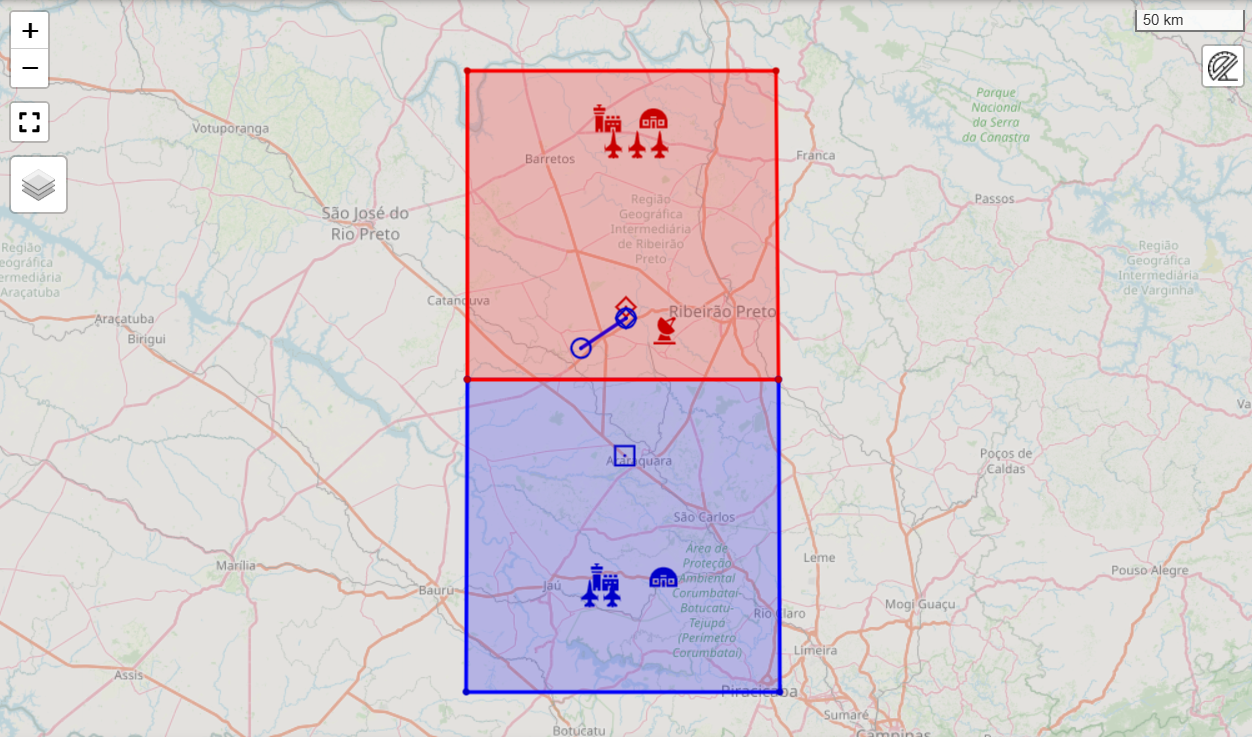
\includegraphics[width=0.82\textwidth]{Cap2/webstation-example.png}
    \caption{Example of a defensive scenario modeled via Webstation.}
    \label{fig:webstation-example}
\end{figure}

Two blue fighters must enter enemy territory, reach designated points, and return successfully. Moreover, three red fighters are activated upon radar detection and engage in combat.

Even in a simple setting such as this one, many analytical questions may arise. For instance, how sensitive is a certain outcome, such as the blue team survival rate, to the radar's longitude? Which variables should be tracked in order to support those comparisons?

This type of scenario is representative of the analytical use case targeted by \gls{asa}. The objective is not merely to run one simulation and inspect it visually, but to run a simulation batch, vary selected parameters, and observe how the outcome changes across runs. This is a analytic-wise problem that heavily benefits from \gls{ms}.

In the workflow considered in this thesis, it is useful to distinguish three levels of analytical output:

\begin{itemize}
    \item A \textit{result} is the raw data produced by an individual simulation run;
    \item A \textit{metric} is a useful quantity derived from a single simulation result;
    \item An \textit{aggregate value} is obtained by combining metrics from all runs in a simulation batch.
\end{itemize}

Also, an \textit{Aggregate Function} may be defined as the function used to obtain the aggregate value from each metric.

In the example provided above \gls{qr} scenario, if we run a simulation batch varying radar longitude in order to evaluate its correlation to the survival time of blue jets:

\begin{itemize}
    \item A \textit{result} may include, for each frame, whether a fighter remains alive, when radar detection occurred, or when a combat event happened;
    \item A \textit{metric} may represent the blue fighter jets' survival time;
    \item An \textit{aggregate value} may be the correlation or even a scatterplot between said survival time and the red team radar's longitude.
\end{itemize}

\section{Distributed Computing}

Distributed Computing is the field of computer science concerned with the execution of computations across multiple interconnected computing nodes that cooperate to solve a common problem. Instead of concentrating processing, memory, and storage resources in a single machine, distributed computing systems partition workloads among several autonomous nodes that communicate through a network and coordinate their actions through message exchange.

A widely adopted definition characterizes a distributed system as a collection of autonomous computing elements that appears to its users as a single coherent system \parencite{steen2016distributed}. This definition highlights two fundamental properties. First, the participating nodes operate independently, each possessing its own processing capabilities, local memory, and execution environment. Second, despite this physical distribution, the system presents a unified view to users and applications, abstracting the complexity of coordination and communication among nodes.

The main motivations for adopting distributed computing include scalability, fault tolerance, resource sharing, and performance improvement. By distributing data and computation across multiple machines, systems can process larger workloads than would be feasible on a single computer while also reducing the impact of individual node failures. These characteristics have made distributed computing a foundational paradigm for modern large-scale infrastructures, including cloud computing platforms, distributed file systems, big data processing frameworks, and high-performance computing environments.

\subsection{Distribution Viability in a Simulation Workflow}

In simulation-related research, distributed computing appears both during simulation execution and during post-processing stages. Simulation workloads can be partitioned across multiple processors or machines to reduce execution time, while large volumes of generated data can be analyzed using distributed frameworks that exploit parallelism and data locality.

In this work, distributed computing is not used to accelerate the simulator itself, but rather to accelerate the analytical processing of the simulator's outputs. The former corresponds to the \textit{Execution Stage}, in which simulations are launched and executed. The latter corresponds to the \textit{Analysis and Aggregation Stage}, in which simulation outputs are processed into metrics and batch-level results.

This distinction is important because the proposed workload is naturally decomposable. A simulation batch consists of many individual runs, and each run generates raw outputs that can first be processed independently to derive metrics and then combined to obtain a batch-level aggregate value. Such a decomposition is structurally compatible with distributed data-processing strategies.

\begin{figure}[ht]
    \centering
    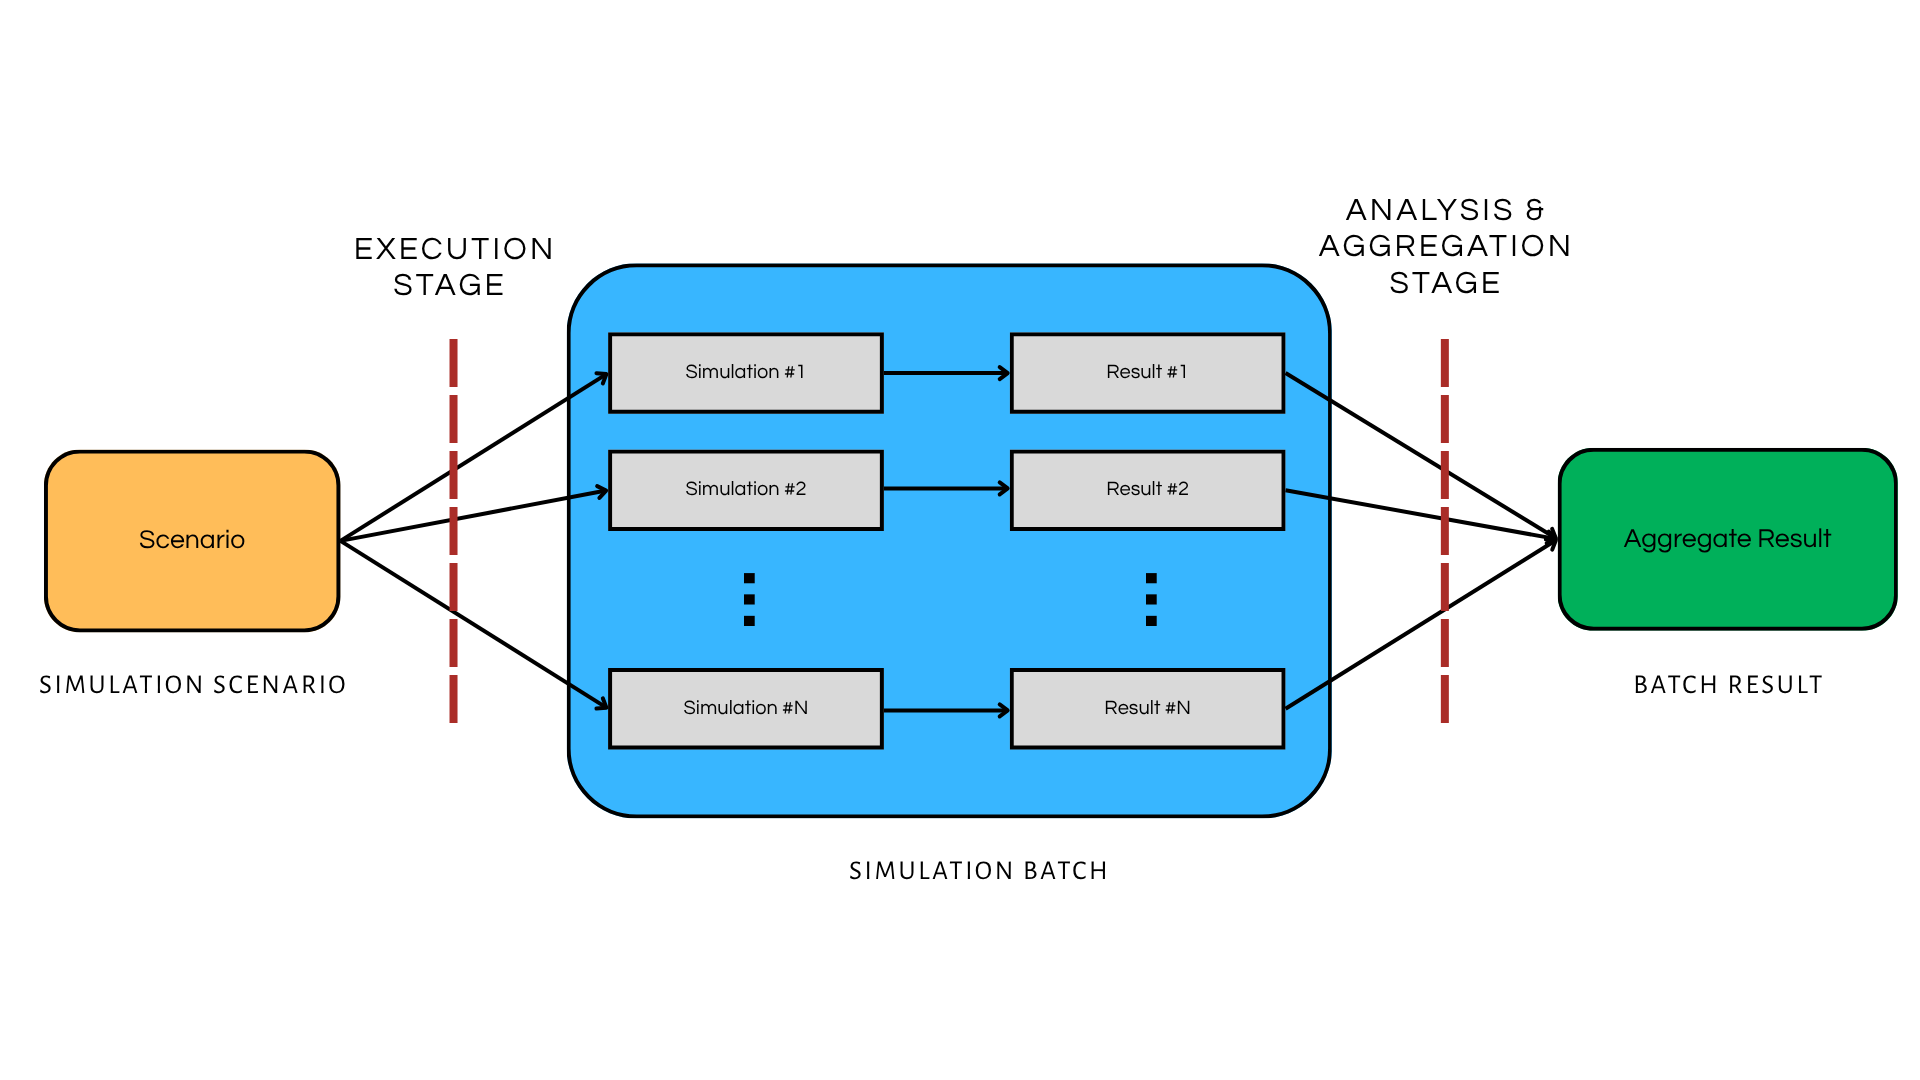
\includegraphics[width=0.82\textwidth]{Cap2/ms-general-pipeline.png}
    \caption{General Pipeline for \gls{ms}, showing both stages: \textit{Execution Stage} and \textit{Analysis and Aggregation Stage}.}
    \label{fig:ms-general-pipeline}
\end{figure}

In the \gls{qr} scenario, considering the metrics are implicit inside \gls{aa} stage in Figure~\ref{fig:ms-general-pipeline}:

\begin{itemize}
    \item The \textit{Scenario} box represents the \gls{qr} Scenario;
    \item Each \textit{Simulation} box represents a different simulation instance. Each simulation:
    \begin{itemize}
        \item starts with a different radar longitude value;
        \item returns if the jets are alive for each simulation frame (value in the \textit{Result} box);
        \item generates the survival time metric at the end;
    \end{itemize}
    \item The \textit{aggregate value} box represents the aggregate value of the metrics. In this case, the aggregate function pairs each metric with the radar longitude for the respective simulation, becoming able to generate for the analyst user:
    \begin{itemize}
        \item the statistical correlation value between both parameters (numerical result);
        \item a scatterplot graphic showing the metrics, in this case, ordered pairs (visual result);
    \end{itemize}
\end{itemize}

Regarding Figure~\ref{fig:ms-general-pipeline} still, although distributed computing can be useful in both stages highlighted in red, this work focuses specifically on the \gls{aa} stage.

This choice is justified by the fact that, historically, the scientific efforts of the high-performance computing community have overwhelmingly focused on optimizing the physical execution time and synchronization of simulation engines (\textit{Execution Stage}) \parencite{fujimoto2016pds}. However, with the exponential growth of data volumes generated by large-scale simulations, the true computational and infrastructural bottleneck has shifted to the subsequent post-processing and metric extraction phases \parencite{valduriez2018scidisc, zheng2021metadata}. Consequently, while the parallel execution of scenarios has reached a high level of maturity, distributed mechanisms tailored for consolidating batch-level analytical results (\textit{Analysis and Aggregation Stage}) still lack standardized approaches, presenting a critical gap in the efficiency of modern scientific workflows.

\subsection{MapReduce}

MapReduce is a distributed programming model that decomposes a computation into two main phases: a \textit{map} phase, in which input records are transformed into intermediate key-value pairs, and a \textit{reduce} phase, in which values associated with the same key are aggregated \parencite{dean2004mapreduce}. Its importance goes beyond one implementation technology: MapReduce offers a conceptual model for thinking about large-scale batch processing over partitioned datasets.

\begin{figure}[ht]
    \centering
    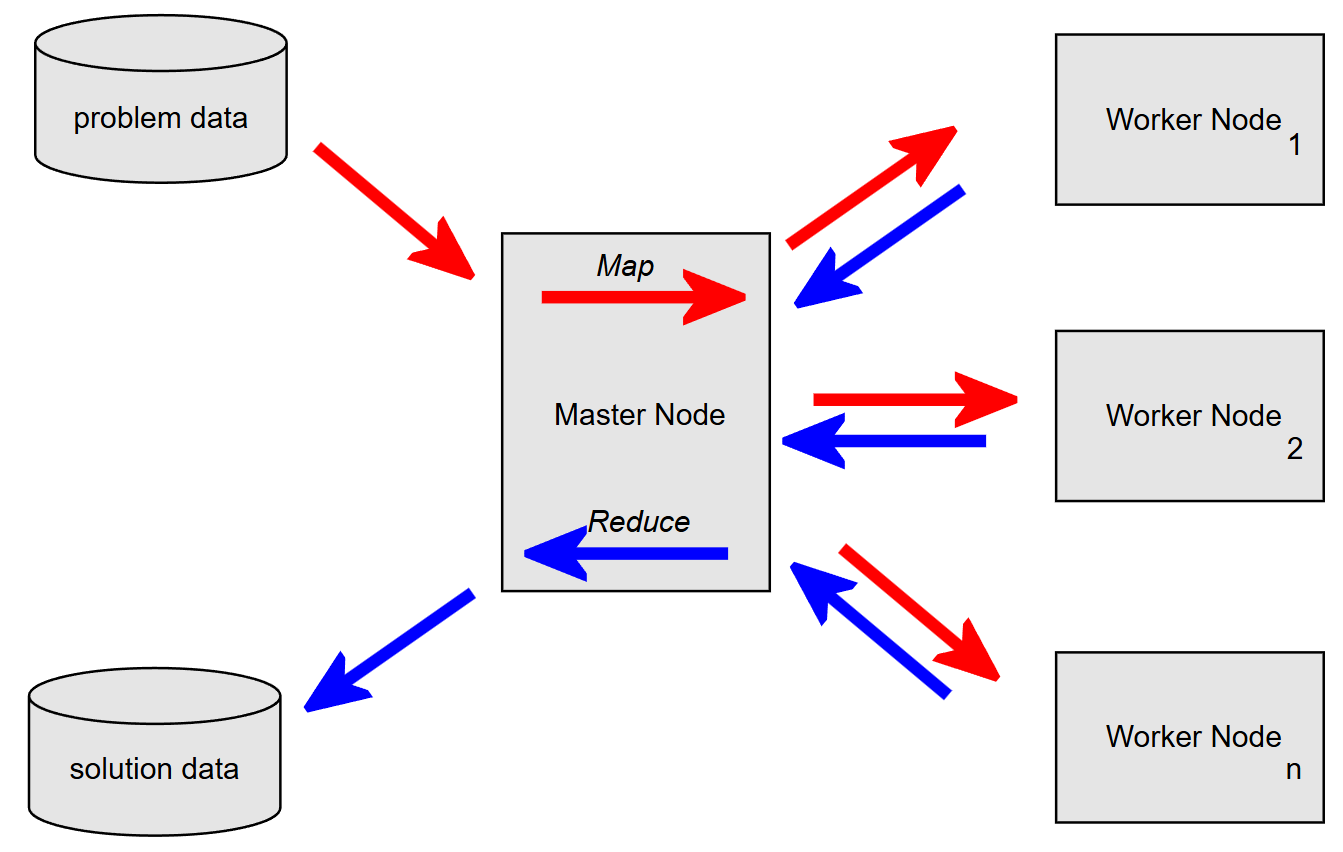
\includegraphics[width=0.82\textwidth]{Cap2/mapreduce-overview.png}
    \caption{MapReduce model overview.}
    \label{fig:mapreduce-overview}
\end{figure}

Figure~\ref{fig:mapreduce-overview} illustrates this model. The computation begins with the \textit{problem data}, representing the input dataset to be processed. A central \textit{master node} receives the job and is responsible for coordinating the execution. During the \textit{map} phase, the master partitions the input data into smaller independent tasks and distributes them among multiple \textit{worker nodes}. Each worker processes its assigned partition in parallel and produces intermediate results. The red arrows in the figure represent the distribution of work from the master to the workers.

Once the mapping tasks have been completed, the intermediate results are returned to the master, as indicated by the blue arrows. During the \textit{reduce} phase, the master combines, aggregates, or summarizes the partial outputs generated by the workers. Depending on the application, this aggregation may involve operations such as summation, counting, averaging, merging data structures, or computing statistical metrics. The final aggregate value is then written to the \textit{solution data}, which represents the output dataset produced by the computation.

Although practical MapReduce implementations often include additional stages such as shuffling, sorting, fault tolerance, and data locality optimization, the fundamental idea remains the same: a master node coordinates a collection of workers that independently process partitions of the input data and subsequently contribute their partial results to a reduction step that generates the final solution. This model enables scalable processing by exploiting parallelism while presenting a relatively simple programming abstraction to the developer.

That conceptual model maps naturally to the problem studied in this thesis. Each simulation output can first be transformed into one or more metrics independently from the others, which resembles the map phase. Then, metrics from all runs in the batch can be combined by an aggregate function, which resembles the reduce phase. Even if the final implementation does not use a canonical Hadoop MapReduce stack, the model remains useful because it provides a clean abstraction for structuring the analytical pipeline.

At the same time, the literature also shows the limits of a purely MapReduce-oriented approach for richer multi-stage analytics. When workflows involve repeated transformations, structured queries, or multiple dependent operations over the same data, models based on richer execution graphs may offer better flexibility and lower overhead \parencite{zaharia2012rdd}. However, these limitations don't pose as a critical problem in our case, since both map and reduce stages can be well translated in our work's analytical pipeline.

\subsection{Apache Spark}

Apache Spark is an open-source distributed computing framework designed for large-scale data processing. Unlike the traditional MapReduce model, which relies on multiple disk-based stages, Spark performs most computations in memory, significantly improving performance for iterative algorithms, interactive analysis, and complex data processing pipelines \parencite{zaharia2012rdd,sparkpysparkdocs}.

Spark organizes computation through a cluster architecture composed of a driver process and multiple worker nodes. Applications are expressed as direct acyclic graphs of transformations and actions, allowing the execution engine to optimize task scheduling, data locality, and fault recovery automatically. The framework also provides a unified ecosystem that includes modules for SQL processing, machine learning, graph analytics, and stream processing, making it suitable for a wide range of data-intensive workloads.

A key advantage of Spark in scientific computing environments is its integration with distributed storage systems such as \gls{hdfs}. By executing computations close to where data are stored, Spark reduces network transfer overhead and enables efficient processing of datasets that exceed the memory and storage capacity of a single machine. These characteristics have motivated its adoption in high-performance computing and large-scale simulation post-processing workflows \parencite{li2018postprocessing}.

\subsection{PySpark}

PySpark is the Python interface to Apache Spark, providing a high-level \gls{api} for distributed data processing while preserving the analytical flexibility expected in Python-based scientific workflows. In this work's context, its adoption is justified because the analysis and aggregation stage can be naturally expressed as distributed transformations and aggregations over simulation outputs, with better scalability than serial post-processing and without requiring the analyst to abandon the Python ecosystem already used in \gls{asa}. In addition, PySpark integrates natively with Hadoop-compatible storage layers, including direct read/write support over \gls{hdfs}, which is consistent with the data-local architecture proposed for reducing transfer overhead and processing large simulation batches efficiently \parencite{zaharia2012rdd,sparkpysparkdocs}.

Finally, related works such as \textcite{li2018postprocessing} reported successful adoption of PySpark combined with \gls{hdfs} for large-scale simulation data post-processing. The study highlights the suitability of Spark's distributed execution model for performing aggregation and analytical operations over datasets that exceed the capacity of a single workstation. The positive results obtained in such environments provide evidence that the Spark-\gls{hdfs} ecosystem constitutes a mature and scalable solution for scientific post-processing workloads.

\section{Distributed File Systems (DFS)}

\gls{dfs} is a storage architecture in which files are partitioned and managed across multiple nodes while being exposed logically as a unified file space. The core motivation of a \gls{dfs} is to improve scalability, availability, and locality of access.

\begin{figure}[ht]
    \centering
    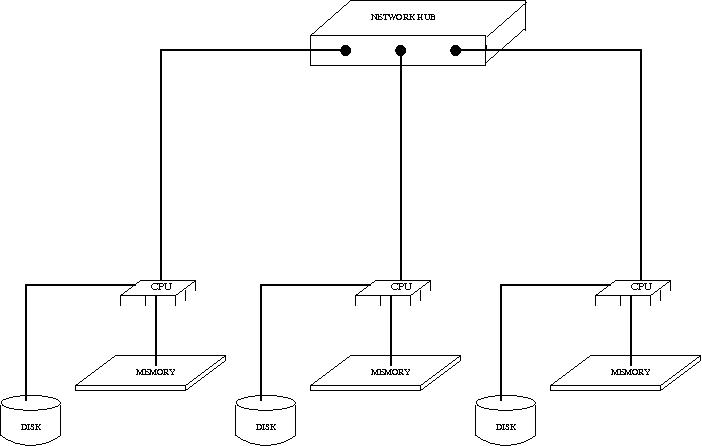
\includegraphics[width=0.82\textwidth]{Cap2/distributed-memory.jpeg}
    \caption{Distributed memory overview.}
    \label{fig:distributed-memory}
\end{figure}

Figure~\ref{fig:distributed-memory} presents a simplified distributed-memory system. Unlike shared-memory architectures, where all processors access a common memory space, each node in a distributed-memory system possesses its own local resources, including a CPU, memory, and persistent storage. The nodes are interconnected through a communication network, represented in the figure by the network hub, which enables data exchange among otherwise independent machines. Because each node maintains its own memory and storage, no processor can directly access the memory of another node; instead, information must be transferred explicitly through network communication.

This organization allows the system to scale by adding new nodes, each contributing additional computational power, memory capacity, and storage resources. The aggregate resources of the cluster can therefore exceed the physical limitations of any individual machine. At the same time, the distributed nature of the architecture introduces challenges related to data placement, communication overhead, consistency, and fault tolerance.

Distributed file systems can be viewed as a software layer built on top of such distributed-memory environments. Rather than exposing separate disks attached to individual nodes, a \gls{dfs} aggregates the storage resources available throughout the cluster and presents them as a unified logical file space. Consequently, applications interact with files as if they were stored in a single system, while the \gls{dfs} transparently manages the distribution, replication, and retrieval of data across the underlying nodes.

The Google File System is a foundational example: it was designed to support very large datasets, tolerate commodity-node failures, and keep computation close to stored data \parencite{ghemawat2003gfs}. These same concerns are relevant because simulation outputs can grow into large collections of batch-generated files whose analytical value depends on efficient retrieval and processing.

For the present work, the relevance of a \gls{dfs} is straightforward. If raw results from many simulations are stored in a distributed file-oriented layer rather than in a single retrieval bottleneck, post-processing can be scheduled close to the output shards themselves. This does not eliminate all communication costs, but it reduces the need to move raw outputs to the analyst before any reduction has occurred. In practical terms, the \gls{dfs} becomes the persistence layer that supports server-side metric extraction and batch-level aggregation.

Considering similar works such as \textcite{li2018postprocessing} and \textcite{morrissey2020velassco}, the \gls{dfs} framework adopted in this work will be \gls{hdfs}, as it provides high-throughput distributed storage, data locality, built-in fault tolerance, and seamless integration with the Hadoop/Spark ecosystem.

\section{Related Work}

The most directly relevant works identified for this thesis are those that address large-scale post-processing of simulation data, distributed scientific analytics, or alternatives to offline post-processing. The comparison developed in this thesis uses criteria that help distinguish both technologies and problem settings:

\begin{itemize}
    \item \textit{Processing paradigm} identifies whether the work relies on hybrid \gls{hpc} and big-data analytics, distributed data platforms, or in-situ / in-transit processing;
    \item \textit{Data access pattern} indicates whether the analysis occurs offline after outputs are persisted, during simulation execution, or through distributed query layers;
    \item \textit{Storage and file format} help reveal whether the solution expects specialized scientific formats, distributed key-value stores, or more generic file-oriented outputs;
    \item \textit{User interface} describes the nature of system access: some systems expose \gls{api}s, while others are designed primarily as infrastructure or embedded analysis layers;
    \item \textit{Primary goal} specifies the system's objective, whether it is scalable post-processing, distributed visualization, workflow automation, or I/O reduction during execution.
\end{itemize}

Together, these criteria make it possible to compare the current \gls{asa} workflow and the proposed TG architecture against the literature on more than one angle.

Tables~\ref{tab:processing_paradigms_a} and~\ref{tab:processing_paradigms_b} summarize the nuances between each study to be mentioned in this section.

\begin{table}[htbp]
    \centering
    \caption{Comparison of related works: processing paradigm, data access, and storage (part~1).}
    \label{tab:processing_paradigms_a}
    \small
    \begin{tabularx}{\linewidth}{l >{\raggedright\arraybackslash}X >{\raggedright\arraybackslash}X >{\raggedright\arraybackslash}X}
        \toprule
        \textbf{Work} & \textbf{Processing Paradigm} & \textbf{Data Access Pattern} & \textbf{Storage / File Format} \\
        \midrule
        Li et al. (2018) & Hybrid \gls{hpc} cluster + Big Data & Simulation output post-processing via \gls{hdfs} & \gls{hpc} outputs \\
        \addlinespace
        Lagares et al. (2022) & Distributed scientific post processing framework & Offline post-processing & \gls{cfd} output formats \\
        \addlinespace
        Morrissey et al. (2020) & MapReduce & Post-processing and distributed querying/visualization & HBase/\gls{hdfs}; large \gls{dem} simulation datasets \\
        \addlinespace
        Friesen et al. (2016) & In-situ / in-transit analysis paradigm & During simulation execution or while data is moving between systems & Simulation data handled inside \gls{hpc} workflow \\
        \addlinespace
        \gls{asa} Project & Centralized post-processing over single storage; serial metric evaluation & Post-processing of already-generated outputs & Single database instance; raw outputs handled as csv files \\
        \addlinespace
        \textbf{This TG proposal} & \textbf{Distributed post-processing architecture} & \textbf{Distributed output post-processing} & \textbf{\gls{dfs} for outputs; distributed storage of batch results/metrics} \\
        \bottomrule
    \end{tabularx}
\end{table}

\begin{table}[htbp]
    \centering
    \caption{Comparison of related works: user interface, primary goal, and simulation domain (part~2).}
    \label{tab:processing_paradigms_b}
    \small
    \begin{tabularx}{\linewidth}{l >{\raggedright\arraybackslash}X >{\raggedright\arraybackslash}X >{\raggedright\arraybackslash}X}
        \toprule
        \textbf{Work} & \textbf{User Interface} & \textbf{Primary Goal} & \textbf{Simulation Domain} \\
        \midrule
        Li et al. (2018) & Jupyter Notebook via JupyterHub & Implement a hybrid workflow that integrates \gls{hpc} and Hadoop/Spark & Molecular simulation \\
        \addlinespace
        Lagares et al. (2022) & Python \gls{api} & Scalable, out-of-core analysis of large simulation results & Turbulent fluid flow / \gls{cfd} \\
        \addlinespace
        Morrissey et al. (2020) & Platform/\gls{api} access layer for queries & Create a platform that enables local processing and results visualization & Discrete Element Method \\
        \addlinespace
        Friesen et al. (2016) & \gls{hpc} analysis framework & Reduce I/O and storage overhead & Cosmological / Astrophysics \\
        \addlinespace
        \gls{asa} Project & \gls{asa} Webstation + JupyterHub + custom local scripts & Execute simulation batches and allow post-processing of results & Aerospace simulation \\
        \addlinespace
        \textbf{This TG proposal} & \textbf{\gls{asa} platform + Python \gls{api}} & \textbf{Parallelize computing of simulation results} & \textbf{Aerospace simulation} \\
        \bottomrule
    \end{tabularx}
\end{table}

\subsection{Related Works Analysis}

Among the selected works, \textcite{li2018postprocessing} and \textcite{lagares2022aquila} are particularly relevant as they explicitly combine high-performance computing with distributed analytics for post-processing, demonstrating that scalable, distributed, and Python-accessible post-processing is itself a research problem worthy of dedicated system design. \textcite{morrissey2020velassco} proposes a distributed platform for post-processing and visualization of extremely large \gls{dem} datasets, embodying the principle of distributing access, analytics, and visualization over large simulation datasets rather than concentrating all work on the client side. In contrast, \textcite{friesen2016insitu} focuses on in-situ and in-transit analysis rather than post-processing over already-persisted outputs, serving as a boundary definition for what this thesis is not attempting. Finally, \textcite{deelman2015pegasus} demonstrates that complex scientific processing pipelines benefit from explicit workflow representations and fault-aware orchestration across heterogeneous computational resources.

The literature reveals a set of gaps that are highly relevant to the \gls{asa} context. First, relatively few works focus on the \gls{aa} stage as an autonomous architectural problem. In many cases, attention is concentrated on simulation execution, workflow orchestration in general, or in-situ analysis embedded in the simulator. Second, the air-defense simulation domain itself is much less represented than fields such as molecular dynamics, \gls{cfd} (Computational Fluid Dynamics), \gls{dem} (Discrete Element Method), or cosmology \parencite{li2018postprocessing,lagares2022aquila,morrissey2020velassco,friesen2016insitu}.

There are also computational gaps. Many proposed solutions assume tight access to the simulator internals or to specialized scientific formats and infrastructures. Fewer works address black-box simulators that already produce persisted outputs and still need an analyst-facing post-processing workflow. Likewise, the literature does not strongly emphasize the combination of distributed storage, batch-level metric extraction, user-defined aggregate functions, and Python-centric interaction as a unified architectural problem.

These observations position the present thesis in a specific setting: distributed post-processing of already-persisted simulation outputs in a scenario-based aerospace-defense environment, with a workflow that remains accessible to the analyst.
